\section{运动的观念}

运动是个让人讨厌的概念,这意味着运动着的物体它即在这里,它又不在这里,我们该如何描述它呢?在我们的日常经验里,运动得足够快的物体,我们是“看不见”的,也“捉不住”,因为物体运动的太快,我们的眼睛还没来得及对它们成像,它们就已经跑掉了。

我们从来没有看见过运动的物体,我们看到的都是静态图像,在某个时刻$t_0$开始,持续了某个特征时间$\Delta t$,在这段特征时间里,物体基本不动,比如物体位置的变化小于人眼的视觉分辨极限,于是我们得到了一幅完全静态的图像。每个物体的边界和位置在我们的眼睛里都有很好的定义。

这是一个很夸张的讨论,并且因为这个讨论涉及视觉的生理问题而,压根就是错误的。人眼(+大脑皮层)不仅仅是接收光信号的器官,同时它还在主动地对光信号进行处理,真实的视觉是人眼(+大脑皮层)主动参与的结果。

但以上讨论还是有益的,比如在生活中有时我们会看不清,不论是看“静”物,还是看“动”物,我们都有可能看不清,不但看不清,我们还特想看清,这时候我们一般会眯起眼睛,使劲盯着自己想看清的东西使劲看,这就是所谓凝视(gaze)。

凝视就是暂时中止人眼(+大脑皮层)主动处理视觉信息,迫使人眼(+大脑皮层)清空成见和既有的算法,完全被动地接受物体发出的光信号,这就是把人眼纯粹当照相机镜头用了。

实际上再怎么盯着看,我们也看不清飞奔骏马的步态或子弹穿透苹果的细节,但人就是对视觉的东西有好奇,越是看不清,就越想盯着看,于是高速照相机取代了我们的眼睛。得到了完全“客观”的图像,这里可完全没有人眼(+大脑皮层)主观的参与。

\begin{figure}[htbp]
\begin{center}
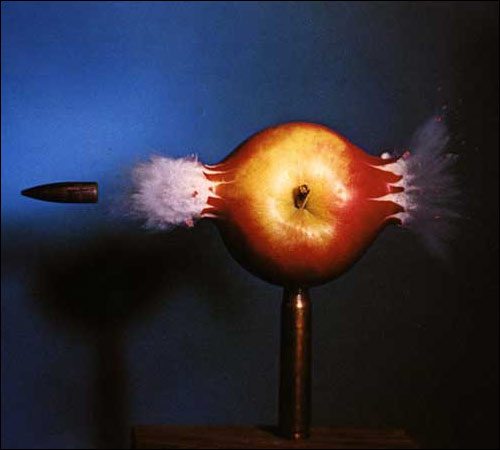
\includegraphics[width=5cm]{Preface/shootapple.jpg}
%\caption{default}
%\label{default}
\end{center}
\end{figure}

人面对运动最终会求助凝视或高速摄像机,说明人是通过“静止”去认识“运动”的,或人压根对“静止”的图像就有偏好,而本能地讨厌“运动”和“变化”,特别是那些无法预知未来的“运动”和“变化”。

\subsection{人对静止图像的偏好}

下面我将举几个例子来说明人对静止图像的偏好,所谓“静止”就是不变化了,我们可以用等式,比例关系等来描述物理规律,而不是用微分方程。

\begin{enumerate}
\item 

阿基米德的杠杆定律:

杠杆定律不讨论杆不平的状况,当杆平的时候,左右两臂的臂长和施加在两臂的力满足以下关系:

\begin{equation}
W_L R_L  = W_R R_R 
\end{equation}

我们可以设想杠杆稍微动起来,比如逆时针转动了$\theta$角度,假设$\theta$很小。

左臂会向下转,角度$\theta$张成的圆弧长度为:

\begin{equation*}
R_L \theta
\end{equation*}

即左侧重物$W_L$会向下移动$R_L \theta$。

重力方向向下,即重物$W_L$移动的方向和重力的方向一致。我们在簿记表中记做“+”,即$W_L$做正功。

\begin{equation*}
W_L  R_L \theta
\end{equation*}

类似地右臂会向上转,角度$\theta$张成的圆弧长度为:

\begin{equation*}
R_R \theta
\end{equation*}

即右侧重物$W_R$会向上移动$R_R \theta $。

重力方向向下,即重物$W_R$移动的方向和重力的方向相反。我们在簿记表中记做“-”,即$W_R$做负功。

\begin{equation*}
W_R R_R \theta
\end{equation*}

根据杠杆定律$W_L R_L  = W_R R_R$,簿记表中的正负贡献正好相抵。

杠杆定律关注的是达到平衡/静止状态的条件。

\item

阿基米德的浮力定律:

物体浸泡在液体中的浮力等于它排开液体的重量。

用今天的物理概念很容易证明。假设一个规则的物体,比如立方体放入水中,或者它比水轻,或者它比水重。

如果它比水轻的话,假设立方体浸入水的深度为$h$,水中压强是各个方向都一样的,并且和深度有关,满足关系:

\begin{equation}
P = \rho_0 g h
\end{equation}

这个压强作用于立方体的底部,方向向上,大小是:

\begin{equation*}
PS = \rho_0 g h S = \rho_0 V g = M_0 g
\end{equation*}

这里$h S$就是排开水的体积,$M_0 g $就是排开水的重量。

假设立方体比水重的证明与之类似,立方体会全部浸入水中,假设上表面距离水面$h$,下表面距离水面为$h + L$。

浮力就是上下表面的压力差,因为作用于下表面的压力较大,所以浮力的方向是向上的。

\begin{equation*}
F = \rho_0 g (h + L) S - \rho_0 g h S = \rho_0 g L S = \rho_0 V g
\end{equation*}

这里$V = LS$是立方体的体积,浮力的大小仍是排开水的重量$\rho_0 V g$。

\item

亚里士多德对运动快慢的讨论:

亚里士多德说重物下落速度较快,轻物下落速度较慢。但亚里士多德讨论的是匀速运动的物体,他其实也注意到物体在刚刚落下的时候运动速度是在变化的,但他拒绝讨论这一阶段,或者说他当时尚不具备讨论速度变化的数学手段。

当重物下落时,由于下落速度$v$的存在,重物会受到一个向上的粘滞阻力。根据斯托克斯定律:粘滞阻力的大小正比于下落速度$v$,此外粘滞阻力也正比于重物的大小,如果是球的话,就正比于球的半径$r$,写成数学式子:

\begin{equation}
F = 6 \pi \eta r v
\end{equation}

这里$\eta$是粘滞系数,和介质及重物的材质有关。实际上空气的粘滞系数比较小,所以重物要下落比较长的距离才会积累到足够大的速度以与重力抵消。为了演示粘滞阻力可以很快抵消掉重力,我们一般都是在粘稠的油中做这个实验,用不同的油,不同直径,不同密度的球来做这个实验。

球的重量可表示为:

\begin{equation*}
Mg = \rho V g = \rho \frac{4 \pi r^3}{3} g
\end{equation*}

考虑到球本身还有浮力$F'$,这个浮力和球排开的流体的重量正好相等。

\begin{equation*}
F' = \rho_0 V g = \rho_0 \frac{4 \pi r^3}{3} g
\end{equation*}

向上的力是浮力$F'$加上粘滞阻力$F$,向下的力是重量$Mg$,我们得到平衡条件:

\begin{equation*}
\rho_0 V g + 6 \pi \eta r v = \rho V g
\end{equation*}

即:

\begin{equation}
( \rho - \rho_0  ) V g = 6 \pi \eta r v
\end{equation}

如果是空气的话,铁球的密度远大于空气的密度,$(\rho - \rho_0) V g = Mg $,就是铁球的重量。球最终匀速落下的速度:

\begin{equation}
v = \frac{Mg}{ 6 \pi \eta r  }
\end{equation}

即物体越重落下的越快。这就是亚里士多德的结论。

必须声明以上讨论是基于现代物理语言和符号的,但这确实是亚里士多德的思路。

\item

最后一个例子是行星运动:

行星运动的轨迹可以是正圆,可以是椭圆,也可以是抛物线,甚至是双曲线(后两种其实已经不是行星了,因为它们注定会飞行到距离恒星无穷远的地方)。

这其实是很复杂的,除正圆的运动外,即行星围绕恒星做正圆的运动是匀速运动,剩下的都不是匀速运动。

我们其实是通过轨迹来理解行星的运动的,不论是椭圆还是双曲线对我们来说都是静态的图形,运动在这里被我们取消了。

当然我们可以指着行星运动的轨迹说,行星离恒星越近它们的速度就越大等等。

比如对椭圆轨道而言,在近日点的速度$v_n$,和在近日点时行星距离恒星的距离$R_n$,与远日点的速度$v_f$,和在远日点时行星距离恒星的距离$R_f$满足:

\begin{equation*}
v_n R_n = v_f R_f
\end{equation*}

\end{enumerate}

\subsection{伽利略的斜面实验}

要想定量地研究运动,必须能对时间进行精确的测定。亚里士多德之所以只研究匀速的运动和他缺乏精确地测量时间的手段有关。

传说,伽利略(1564 — 1642)为了反驳亚里士多德的落体理论,曾登上55米高的比萨斜塔做了著名的落体实验。但这听上去更像是个表演,类似马戏团的表演,因为它仍然缺乏测量和数据的支撑。

我们可以估算一下落体从55米高落下需要多少时间。

\begin{equation}
s = \frac{1}{2} g t^2
\end{equation}

这里$g = 9.8 m/s^2$是地球表面的重力加速度。解出:

\begin{equation*}
t = \sqrt{\frac{2 s}{ g}} = 3.35(s)
\end{equation*}

即大约只需要3秒,要精确地测量这个时间在伽利略的时代是很困难的。这就需要发挥高超的实验技艺将问题转化。

伽利略到底有没有到比萨斜塔去作秀我们不知道,但伽利略确实做过一个“斜面落体实验”。

\begin{itemize}
\item 

首先取来一个长约7米的木板,在木板上刻一条一指宽的槽,槽要非常直而且平滑。

\item

把木板倾斜放置,让一个坚硬、光滑的黄铜球沿木板上的槽滚落。

让铜球沿倾斜放置的木板滚下来是可以有效地减小加速运动的加速度的。这当然会减轻精确测量时间的压力。

\item

在伽利略的时代最精确的测量时间的装置是水钟。

水钟有巨大的装水容器,水会从容器底部的细管流出,由于装水容器的横截面积很大,我们可以忽略水面高度的变化,只要细管的管口经过精细的打磨和加工,经细管流出水的速度就是恒定的。

水钟可以非常精确地计时,这是伽利略斜面实验得以完成的前提。

\item

让铜球从斜面上滚落,开始滚动的瞬间我们打开水钟,当球运动到特定的位置,比如:10厘米,20厘米,30厘米,……我们关掉水钟。

我们把水钟里流出的水收集起来,然后通过非常精密的天平(杠杆原理)去测量它们的质量,水的质量是正比于——铜球滚落特定距离——所用时间的。

\end{itemize}

其实水钟也是希腊-罗马时代的发明,原则上说古典时代人们也是可以做伽利略的“斜面实验”的。

对此我的评论是:(1)首先我们需膜拜伽利略构思实验之精妙;(2)其次即便某位哲学家在2000多年前就做过“斜面实验”,但他也不会有效地撬动当时主流的思想,因为孤立的一个实验(或理论)并没有多少意义,必须把它放入一个潮流里,它的意义才会显现出来。(3)伽利略的这项工作是近代物理学一系列工作最开始的几个之一。评价一项实验,一个工作,重要的是看它引发了什么。

在伽利略的手稿中,我们发现了这么一个表格:

\begin{table}[htdp]
\caption{伽利略的斜面实验记录}
\begin{center}
\begin{tabular}{|c|c|c|}
\hline
$t^2$ & t & s \\
\hline
1 & 1 & 32 \\
4 & 2 & 130+ \\
9 & 3 & 298+ \\
16 & 4 & 526+ \\
25 & 5 & 824 \\
36 & 6 & 1192 \\
49 & 7 & 1600 \\
64 & 8 & 2104 \\
\hline
\end{tabular}
\end{center}
\label{default}
\end{table}%

表格中第三列是距离,单位不是很清楚,但想必是在他7米长的大斜面上做的。第二列是时间,这个时间倒不一定是用水钟测量的,因为它是1、2、3……罗列的,很有可能是人的脉搏或单摆。

第一列数字是后加上去的,因为笔迹的颜色不一样,看来伽利略猜测到这里面的规律了,即铜球延斜面滚落的距离$s$正比于所需时间$t$的平方。

\begin{equation}
s \propto t^2
\end{equation}

可以想象当伽利略达到这个猜测后,他就可以利用水钟做更精确的实验以验证这一结果。比如他可以让铜球延斜面滚落:10厘米,40厘米,90厘米,160厘米,……以验证它们对应的滚落时间是否接近于:$1: 2^2: 3^2 : 4^2 : ...$

\subsection{微分}

用现代的语言,伽利略发现的规律是,

\begin{equation}
s(t) = \frac{1}{2} a t^2
\end{equation}

即加速度恒定条件下,物体的运动。

对这种运动速度是时时刻刻变化的。此时再把速度$v$定义成距离和时间之比就不合适了。

\begin{equation}
v = \frac{s}{t}
\end{equation}

由伽利略测出的数据,我们有一种直觉,即运动速度是越来越快的。我们现在用对距离的微分来定义速度:

\begin{equation}
v = \frac{d s}{d t } = \lim\limits_{\Delta t \to 0} \frac{s(t + \Delta t) - s(t)}{\Delta t}
\end{equation}

这里的$\lim\limits_{\Delta t \to 0}$表示一个取极限的过程,即构造一个序列:$\Delta t = 1 s, 0.1 s, 0.001s , ...$用越来越小的时间间隔去反复计算$\frac{s(t + \Delta t) - s(t)}{\Delta t}$,看什么时候商的取值会稳定下来。这个其实就是做工程的思路,关注结果,不关心形式是否优美。

或者我们把分子展开:

\begin{equation*}
s(t + \Delta t) - s(t) = \frac{a}{2} \left( t^2 + 2t \Delta t + (\Delta t)^2 - t^2 \right)
\end{equation*}

考虑到$ \Delta t \to 0 $是个很小很小的数,那么$( \Delta t )^2$是个更小更小的数,我们管$(\Delta t) ^2$叫高阶无穷小,在有低阶无穷小项$2 t \Delta t$存在的情况下,我们可以放心地忽略$( \Delta t )^2$。


现在公式变成了:

\begin{equation*}
v(t) = \frac{a}{2}  \cdot  \frac{2t \Delta t}{\Delta t } = at
\end{equation*}

现在速度确实变成一个和时间$t$有关的函数。即速度在时时刻刻地变化着。

以下罗列求微分运算的主要结果:

\begin{enumerate}
\item 

对幂函数$x^n$求微分,假设这里$n > 0$,并且是整数。

求微分也叫求导,记做$(x^n)'$

\begin{equation}
( x^n )' = \lim\limits_{\eta \to 0} \frac{(x+ \eta)^n - x^n}{\eta}
\end{equation}

这里需要计算$(x + \eta)^n$

\begin{eqnarray*}
( x + \eta)^n & = & (x + \eta)(x + \eta) ... (x + \eta)   \\
{} & = & x^n + n x^{n-1} \eta + \frac{n(n-1)}{2} x^{n-2} \eta^2 + ... + \eta^n
\end{eqnarray*}

这里涉及$n$个$( x + \eta)$连乘,

\begin{itemize}
\item 

第一项自然是$x^n$;

\item

第二项是一阶无穷小,即包含$\eta$的项,这意味着要从$n$个$( x + \eta)$中挑出一个$\eta$来,这有$n$种可能性;

\item

接下来的一项,是包含$\eta^2$的项,这意味着要从$n$个$( x + \eta)$挑出两个$\eta$来,但这个挑选和次序无关,因此有$\frac{n (n -1)}{2}$。

即第一次挑选有$n$种可能性,第二次挑选只能从剩下的$n-1$项里选,因此有$n-1$种可能性,$n(n-1)$是考虑挑选次序的,即认为先选第一项再选第二项,和先选第二项再选第一项是两种情形,但在我们这里与次序无关,因此需要再除以2。

\item

一般地,包含$\eta^m$的项,其系数是$\frac{n(n-1)...(n-m+1)}{m!}$

这里$m!$被定义为:

\begin{equation}
m! = m (m-1) (m-2) ... 3 \cdot 2 \cdot 1
\end{equation}

即$m$个不同的人排队,从左排到右的所有方式数,先是从$m$个人里随便挑一个出来,排第一个儿,有$m$种可能性,然后在剩下的$(m-1)$个人挑一个出来排第二个儿,有$m-1$种可能性……


\item

最后一项,包含$\eta^n$的项,其系数是$\frac{n!}{n!} = 1$

\end{itemize}

现在我们可计算出$x^n$的导数是:

\begin{equation}
(x^n)' = \lim\limits_{\eta \to 0} \frac{n x^{n-1} \eta}{\eta } = n x^{n-1} 
\end{equation}

\item

我们定义一个新的函数$e^x$

\begin{equation}
e^x = \sum\limits_{n=0}^{\infty} \frac{x^n}{n!} = 1+x + \frac{x^2}{2} + ...
\end{equation}

可以证明$e^x$的导数还是它自己。

\begin{eqnarray*}
(e^x)' & = & ( 1 + x + \frac{x^2}{2} +  \frac{x^3}{3!} +... + \frac{x^n}{n!}  +... )' \\
{} & = & 1 + x + \frac{x^2}{2} + ... + \frac{x^{n-1}}{(n-1)!} + ...
\end{eqnarray*}

那么$e$等于多少呢?

我们取$x =1$,会得到一个估算$e$的数列求和:

\begin{equation}
e = 1 + 1 + \frac{1}{2!} + \frac{1}{3!} + ... + \frac{1}{n!} + ...
\end{equation}

我们管$e$叫做自然指数,也叫欧拉数(Euler's Number),它大约是:

\begin{equation}
e \approx 2.71828
\end{equation}

很重要地,$e^x$的导数还是$e^x$

\begin{equation}
(e^x)' = \frac{d}{dx} e^x = e^x
\end{equation}

\item

假设$f(x)$和$g(x)$是两个函数,存在微分$\frac{df}{dx}$,$\frac{dg}{dx}$,对函数$f(g)$求微分:

\begin{equation}
\frac{d f(g)}{d x} = \frac{d f}{d g} \frac{d g}{ d x}
\end{equation}

作为一个简单的例子,对$f(ax)$求微分:

\begin{equation}
\frac{d f(ax)}{d x} = a \frac{d f(x)}{ d x} 
\end{equation}

\item

假设$f(x) = u(x) v(x)$,导数$u'$, $v'$都存在,求$f'$

\begin{eqnarray*}
f' & = & \lim\limits_{\eta \to 0} \frac{ u(x+\eta) v (x+ \eta) - u(x) v(x) }{ \eta } \\
{} & = & \frac{  u(x+\eta) v (x+ \eta) - u(x+\eta) v + u(x+\eta) v - u v  }{\eta} \\
{} & = & u'v + u v'
\end{eqnarray*}

即:

\begin{equation}
( u v)' = u' v + u v'
\end{equation}

\item

函数$y = f(x)$是由$x \to y$的映射$f$,我们也可定义逆映射$f^{-1}: y \to x$,记做:$x = f^{-1}(y)$。

假设存在导数$f'$,逆函数$(f^{-1})'$的导数如何表示?

\begin{equation*}
\left(  f^{-1} (y) \right)' = \frac{dx}{dy} = \frac{1}{dy/dx} = \frac{1}{ f'(x) }
\end{equation*}

但我们现在必须把右侧的变量$x$变为以$y$为变量,即需代入:$x = f^{-1} (y)$

\begin{equation*}
\left(  f^{-1} (y) \right)' = \frac{1}{ f'( f^{-1} (y)) }
\end{equation*}

然后我们再把等式左侧和右侧的变量都改变为$x$,

\begin{equation}
\left(  f^{-1} (x) \right)' = \frac{1}{ f'( f^{-1} (x)) }
\end{equation}

作为一个例子,我们来研究一下$e^x$的逆函数:

\begin{eqnarray*}
y &=& e^x \\
x &=& \ln y
\end{eqnarray*}

即:

\begin{eqnarray*}
\ln e^x & = & x \\
e^{\ln y} & = & y
\end{eqnarray*}

现在来计算$(\ln y )'$

\begin{equation*}
( \ln y)' = \frac{1}{dy/dx} = \frac{1}{e^x} = \frac{1}{e^{\ln y}} = \frac{1}{y} 
\end{equation*}

最后我们把$y$换成$x$,

\begin{equation}
( \ln x)' = \frac{1}{x}
\end{equation}

\item

考虑函数$f(x) = \frac{u(x)}{v(x)}$,假设导数$u'$, $v'$存在,求导数$f'$。

根据微分/导数的定义:

\begin{equation*}
f' = \lim\limits_{\eta \to 0} \frac{1}{\eta} \left( \frac{u(x+\eta)}{v(x+\eta)} - \frac{u}{v} \right)
\end{equation*}

其中:

\begin{equation*}
\frac{u(x+\eta)}{v(x+\eta)} - \frac{u}{v} = \frac{ u(x+\eta) v - u v(x+\eta)  }{ v(x+\eta) v }
\end{equation*}

其中:

\begin{eqnarray*}
u(x+\eta) v - u v(x+\eta) & = & u(x+\eta) v - uv + u v - u v(x+\eta) \\
{} & = & (u(x+\eta)-u)v - u(v(x+\eta)-v )
\end{eqnarray*}

因此:

\begin{equation}
\left( \frac{u}{v} \right)' = \frac{ u' v - u v' }{v^2}
\end{equation}

现举一例:

比如我们计算$\frac{1}{x}$的导数$\left( \frac{1}{x} \right)'$

\begin{equation*}
\left( \frac{1}{x} \right)' = \frac{ - 1 }{x^2} = -x^{-2}
\end{equation*}

类似地,我们可得到$\frac{1}{x^n} $的导数:$\left( \frac{1}{x^n}  \right)'$

\begin{equation}
\left( x^{-n} \right)' = -n x^{-(n+1)}
\end{equation}

\item

现在来求正弦函数$\sin x$的导数,根据定义:

\begin{equation*}
( \sin x)' = \lim\limits_{\eta \to 0} \frac{ \sin (x + \eta) - \sin x }{\eta}
\end{equation*}

$\sin (x + \eta)$可展开为:

\begin{equation*}
\sin (x + \eta) = \sin x \cos \eta + \cos x \sin \eta
\end{equation*}

当$\eta \to 0$时,$\cos \eta \to 1$,$\sin \eta \to \eta$

因此:

\begin{equation}
( \sin x)' = \cos x
\end{equation}

类似地,我们可以证明余弦函数$\cos x$ 的导数:

\begin{equation}
( \cos x )' = - \sin x
\end{equation}

\item

泰勒展开:

假如对函数$f(x)$,我们求出了其一阶导数$f'$,然后继续求出了二阶导数$f''$($f''$就是$f'$的导数),这个过程可以一直进行下去,……,比如$f$的第$n$阶导数表示为$f^{(n)}$

我们可以把$f(x)$在$f(0)$附近展开为一个级数求和的形式:

\begin{equation}
f(x) = f(0) + f'(0)x+ \frac{f''(0)}{2}x^2 + ... + \frac{f^{(n)} (0) }{n!} x^n + ...
\end{equation}

由于$(e^x)' = e^x$,并且$e^0 = 1$,$e^x$可表示为:

\begin{equation}
e^x = 1 + x + \frac{x^2}{2} + ... + \frac{x^n}{n!} + ...
\end{equation}

由于$(\sin x)' = \cos x$,$(\cos x)' = -sin x$,并且$\sin 0 = 0$, $\cos 0 = 1$,我们可以得到$\sin x$和$\cos x$的展开式:

\begin{eqnarray*}
\cos x &=& 1 - \frac{x^2}{2} +  ... + (-)^n \frac{x^{2n}}{(2n)!} + ... \\
\sin x &=& x - \frac{x^3}{3!} +  ... + (-)^n \frac{ x^{2n+1} }{(2n+1)!} + ...
\end{eqnarray*}

\end{enumerate}

%%%%

\subsection{原子的半衰期}

$y = e^x$是很多微分方程的解。现举一例:

考虑放射性衰变,初始时刻$t = 0$,有$N_0$个放射性原子,放射性原子可能发生衰变,通过某过程变成其他原子,考虑某个时刻$t$,有多少原子会发生衰变呢?

发生衰变的数目记做$d N$,它正比于此时此刻放射性原子的总数目$N(t)$,也正比于时间间隔$d t$,由于原子会衰变为其他原子,这是个减少的过程,因此$d N$是负的,综上所述,我们会得到一个描述这样过程的微分方程:

\begin{equation}
d N = - \alpha N dt
\end{equation}

这里的$\alpha$是衰变因子,对不同的放射性原子它的取值可以不一样。

那么$N(t)$随时间变化的规律是什么呢?

解:

首先把$N$移到等式的左边:

\begin{equation*}
\frac{dN}{N} = - \alpha dt
\end{equation*}

考虑到

\begin{equation}
\frac{d \ln x}{ d x} = \frac{1}{x}
\end{equation}

这意味着:

\begin{equation}
\frac{d x}{x} = d ( \ln x )
\end{equation}

因此:

\begin{equation*}
\frac{dN}{N} = d ( \ln N  ) = - \alpha dt
\end{equation*}

对$d (\ln N)$积分,从$0 \to t$,得到:

\begin{equation*}
\ln N(t ) - \ln N_0 = \ln \frac{N(t)}{N_0}  = - \alpha t
\end{equation*}

因此:

\begin{equation*}
\frac{N(t)}{N_0} = e^{- \alpha t}
\end{equation*}

即:

\begin{equation}
N(t) = N_0 e^{- \alpha t}
\end{equation}

我们也把$\alpha$改写为$\frac{1}{\tau}$,这样:

\begin{equation}
N(t) = N_0 e^{- \frac{t}{\tau}}
\end{equation}

当$t = \tau$时,

\begin{equation}
N(\tau) = N_0 e^{-1}
\end{equation}

即粒子数会衰减为原先的$e^{-1} = 0.368$,即原先的大约1/3。我们管$\tau$叫寿命。

还有所谓半衰期,即当$t$等于多少时,$\frac{N(t)}{N_0} = \frac{1}{2}$

\begin{equation*}
\ln \frac{1}{2} = - \ln 2 = - \frac{t }{\tau} 
\end{equation*}

解出:$t = t_{1/2} = \ln 2 \tau = 0.693 \tau$。

\begin{table}[htdp]
\caption{原子的半衰期}
\begin{center}
\begin{tabular}{|c|c|}
\hline
碳14 & 5730年  \\
铀235 & 7.1亿年 \\
铀238 & 45亿年 \\
\hline
\end{tabular}
\end{center}
\label{default}
\end{table}%



%%%%


\subsection{量纲}


只有同类的量才能相加。比如:

\begin{center}
1苹果 + 1鸭梨
\end{center}

是没有意义的。

说:

\begin{center}
1苹果=1鸭梨
\end{center}

也是没意义的。

但,

\begin{center}
1水果 + 1水果 = 2水果
\end{center}

就有意义。

我们管1叫数字,苹果叫单位,[苹果]叫量纲。

我们用单位来表示“类”,比如1苹果就是一个单位,而1鸭梨是另一个单位。我们对相等的规定是数字和数字相同,而表示“类”的单位也要和单位一样。

英文的量纲是dimension,dimension有尺寸和维度的意思。在$x$方向上我们可以向前也可以向后,但我们还有$y$方向,和$x$方向完全无关,这是另一个维度,维度的扩张和乘法有关。

乘法的定义是这样的:

\begin{center}
1苹果 x 2鸭梨 = 2 苹果·鸭梨
\end{center}

即数字和数字乘,单位和单位乘,所谓单位和单位乘就是把苹果和鸭梨并列,得到新的类,或新的单位——“苹果·鸭梨”,苹果·鸭梨的量纲是:

\begin{center}
[苹果·鸭梨] = [苹果] x [鸭梨]
\end{center}

举例而言,物理里面功的定义是:

\begin{equation}
W = F_l \cdot l
\end{equation}

功是力$F$乘位移$l$,功的单位是焦耳,功的量纲是:

\begin{center}
[功] = [力] x [长度]
\end{center}

我们希望把任意物理量的量纲都表示为几个基本物理量的量纲的表达,在力学中我们选:长度、质量和时间。

那么力的量纲是什么呢?

由牛顿第二定律:

\begin{equation}
F = m a
\end{equation}

力的量纲是:

\begin{center}
[力] = [质量] x [加速度]
\end{center}

加速度的定义是:

\begin{equation}
a = \frac{d v}{d t} = \frac{d^2 x}{dt^2}
\end{equation}

加速度的量纲是:

\begin{center}
[加速度] = [长度] [时间]$^{-2}$
\end{center}

因此功的量纲是:

\begin{center}
[功] = [质量] [长度] [时间]$^{-2}$ [长度] = [质量] [长度]$^2$ [时间]$^{-2}$
\end{center}

我们可以证明功的量纲和动能的量纲是一样的,它们是同一类的物理量。

动能的定义是:

\begin{equation}
K = \frac{m v^2}{2}
\end{equation}

动能的量纲是:

\begin{center}
[动能] = [质量] [长度]$^2$ [时间]$^{-2}$
\end{center}

弧度是没有量纲的,这与我们对弧度的定义有关。

考虑一段圆弧,圆弧所对的角度是$\theta$,或说我们由角度$\theta$,半径$R$,得到一段圆弧,假设圆弧的长度是$L$。

圆弧长度$L$正比于角度$\theta$,也正比于半径$R$,

我们定义:

\begin{equation}
L = R \theta
\end{equation}

圆弧$L$和半径$R$的量纲都是长度。这样定义的角度$\theta$是无量纲的。

更多例子:

\begin{enumerate}
\item 

5米 x 6米 = 30 米·米

“米·米”和“米”不是一类的,我们管“米·米”叫面积,而“米”叫长度。


\item

0.1 元 x 0.1 元 = 0.01 元·元

“元”是货币单位,“元·元”和“元”不是一类的,0.01自然不是对货币多少的度量。

\item

在物理中还会出现这样的表达,比如:

\begin{equation*}
A e^{i (kx - \omega t)}
\end{equation*}

这里在$e$指数里面,$kx - \omega t$ 解释为角度,是无量纲的。

$x$的量纲是[长度],$k$波矢的量纲是[长度]$^{-1}$

波矢的定义是:

\begin{equation*}
k = \frac{2 \pi}{ \lambda}
\end{equation*}

即空间上每增加长度份额$\lambda$,相位(无量纲)会增加$2 \pi$,即重复一周期重回起点。

\item

对包含$e$指数的物理公式,考虑到:

\begin{equation*}
e^x = 1 + x + \frac{x^2}{2} + \frac{x^3}{3!} + …
\end{equation*}

$x$只能是无量纲的,$e^x$也是无量纲的,否则就会造成$e^x$有不确定的量纲,这是不可能的。

比如(放射性)衰减公式:$N(t) = N_0 e^{- t / \tau}$,$t$的量纲是[时间],$\tau$的量纲也是[时间],我们把$\tau$解读为“寿命”。


\end{enumerate}


\subsection*{练习}

请证明量子普适电导率$\frac{e^2}{h}$的量纲是电导率的量纲,这里$e$是电子的电荷,$h$是普朗克常数。